\section{Forgetting Requires Remembering Why}
\label{sec:theory}

\begin{figure*}[t]
  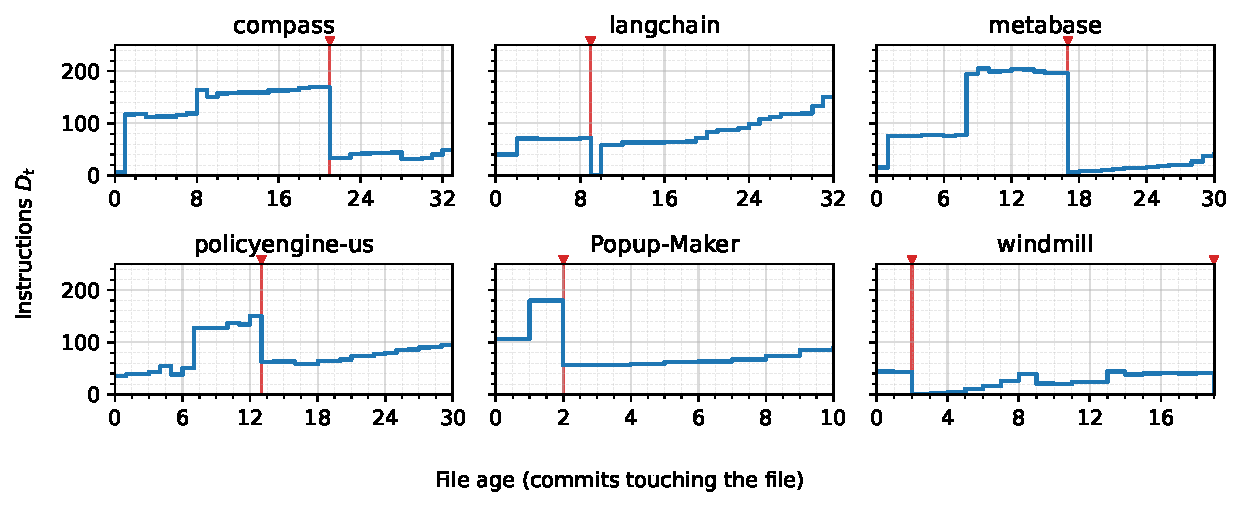
\includegraphics[width=\linewidth]{assets/fig_mass_rewrite_examples.pdf}
  \caption{
    Maintainers bulldoze rather than prune, and the ratchet
    survives it. Instruction count $D_t$ for six illustrative context
    files; a red rule marks a commit cutting the file to at most half its
    instructions. Wholesale rewrites carry \RewriteDeathShare{} of all
    instruction deaths, and regrowth is immediate: the mean file drops to
    \RewriteDropPct{} and is back to \RewriteReboundPct{} within
    \RewriteEventWindow{} commits (\RewriteEventFiles{} files aligned on
    their first rewrite, \autoref{fig:massrewrite:event}).
  }
  \label{fig:massrewrite:examples}
\end{figure*}


We model prompt maintenance as the \emph{online estimation of an unobservable
constraint set from censored, noisy feedback}, and derive an equilibrium prompt size that diverges as
write-time provenance decays. Without that provenance, the optimal estimator becomes append-only.

A task $j = (o_j, C_j)$ pairs a stated objective $o_j$ with its unobservable constraints $C_j \subseteq C$,
which are drawn from a fixed hidden set $C = \{g_c\}$ of verifiers. The prompt at time $t$ is a finite set of
instructions $D_t$, with instruction $d$ entering the prompt at time $\tau_d$ and having age $a_d = t -
\tau_d$. A response to $j$ satisfies $c \in C_j$ with probability $q_c(D, j)$; $C$ is unobservable except for
draws from $q_C$.

At each timestep $t$, three parties interact in the system. A (possibly agentic) \emph{maintainer} adds and
deletes instructions, updating the prompt $D_t$. The \emph{harness} draws tasks $j$, runs them using the
\emph{executor} under prompt $D_t$, and then verifies them using $C_j$, generating draws from $q_C$.

A maintainer's target is the \textbf{minimum cover} $D_\star$, the smallest instruction set that maximizes
expected constraint satisfaction. Formally,
\begin{equation}
  \begin{split}
    D_\star &= \operatorname*{argmin}_{D \in \mathcal{M}} |D|, \\
    \mathcal{M} &= \operatorname*{argmax}_{D}\, \mathrm{E}_{j,\,c \in C_j}[q_c(D, j)]
  \end{split}
\end{equation}
Every experiment in this paper scores $D_t$ against $D_\star$ on two axes: \emph{correctness}, the expected
satisfaction $\mathrm{E}[q_c]$, and \emph{excess size}, $\frac{|D_t|}{|D_\star|} - 1$. A maintenance regime
wins only by improving one axis without degrading the other.\looseness=-1

Without assuming a particular functional form, we assume $q_C$ meets the properties listed in
\autoref{tab:characteristics}. Properties A1–A3 (instructability, interference, and redundancy) set the
overall regime whereas properties A4 (censoring) and A5 (stochasticity) respectively block deletions and
drive additions.\looseness=-1

\begin{table}[t]
  \centering\small
  % Narrow label column: @{\hspace{0.6em}} trims the gap after it. tabularx spans the full
  % \columnwidth, with the X (Behavior) column absorbing exactly the width the label and
  % property columns leave over — no hand-tuned fraction to drift when a cell's text changes.
  \begin{tabularx}{\columnwidth}{@{}l@{\hspace{0.6em}}l>{\raggedright\arraybackslash}X@{}}
    \toprule
    & \textbf{Property} & \textbf{Behavior} \\
    \midrule
    A1 & instructability & some $d$ raises $q_c$ \\
    A2 & interference & adding $d$ lowers other $q_{c'}$ \\
    A3 & redundancy & a second $d'$ adds no $q_c$ \\
    A4 & censoring & outcomes don't name their $d$ \\
    A5 & stochasticity & $q_c < 1$ even when covered \\
    \bottomrule
  \end{tabularx}
  \caption{
    The five characteristics of the hidden constraint set and its feedback (\autoref{sec:theory}).
    Instructability, interference and redundancy set the regime axis; censoring blocks deletions;
    stochasticity drives additions.
  }
  \label{tab:characteristics}
\end{table}


Deleting instructions without risking a regression requires a maintainer to run an infeasible number of
counterfactuals. Write $d$'s contribution to $c$ as $\Delta_c(d \mid D) = \mathbb{E}_j[q_c(D, j) - q_c(D
\setminus \{d\}, j)]$ over tasks with $c \in C_j$; $d$ is \emph{excess} when $\Delta_c \le 0$ for every $c$.
Estimating it means probing $D \setminus \{d\}$, and redundancy defeats one-at-a-time probes: two instructions
covering one constraint each look free alone, though deleting both breaks it. An honest audit therefore costs
$O(2^{|D_t|})$ subset probes, and $D_\star$ is incomputable in general. Knowing why a maintainer added $d$ ---
its \emph{latent reasoning} $r_d$ --- collapses that to $O(1)$, but $r_d$ rapidly decays with
$a_d$.\looseness=-1

\begin{figure}[t]
  \centering
  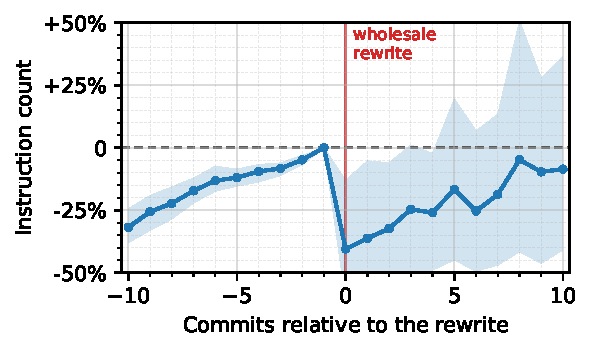
\includegraphics[width=\columnwidth]{assets/fig_mass_rewrite_event.pdf}
  \caption{
    The ratchet: a rewrite resets a prompt's size but not its growth rate. Prompts grow
    \RewriteGrowthPreCommit{} per commit before their first rewrite, are cut to \RewriteDropPct{}, then
    regrow immediately and faster, at \RewriteGrowthPostCommit{} per commit. Mean instructions
    relative to the \emph{first} pre-rewrite, each file's rewrite event aligned to $t=0$; band: 95\%
    bootstrap CI.
  }
  \label{fig:massrewrite:event}
\end{figure}

\begin{figure}[t]
  \centering
  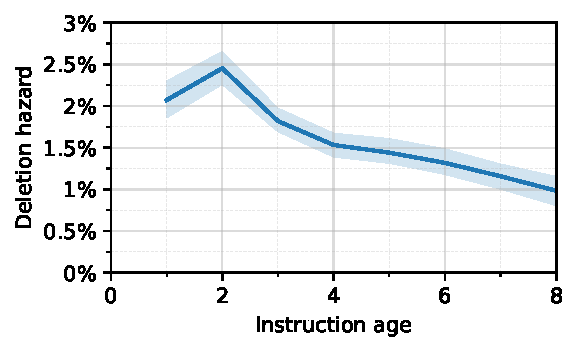
\includegraphics[width=\columnwidth]{assets/fig_hazard_curve.pdf}
  \caption{Deletion hazard \emph{falls} with instruction age: the
    imperfect-recall signature, which instruction staleness (rising) and
    age-independent deletion (flat) both miss. Nelson--Aalen over \FieldDeletions{}
    deletions against age in commits, 95\% repository-stratified bootstrap
  band; slope $\FieldSlopeCommit$/commit ($\FieldSlopeCommitCI$).}
  \label{fig:hazard}
\end{figure}


Recoverability thus sets equilibrium size. Define the decay
\begin{equation}
  \rho(d, a) = \Pr(r_d \text{ recoverable at age } a),
\end{equation}
with marginal $\bar \rho(a) = \mathbb{E}_d\,\rho(d, a)$; thus, $\rho(d, 0) = \bar \rho(0) = 1$ and both $\rho(d,
a) \rightarrow 0$ and $\bar \rho(a) \rightarrow 0$ as $a \rightarrow \infty$. We call that decay
\textbf{imperfect recall}: the instruction stays and its failures recur, but its latent reasoning is
increasingly unrecoverable. A maintainer rationally deletes an instruction only when that reason survives and
it verifies as excess, so the hazard in its own age factorizes (the event-history form used for written
organizational rules; \citealp{schulz1998limits, march2000dynamics, zhou1993dynamics}),
\begin{equation}
  h(a) \;\approx\; \bar \rho(a)\, s(a),
  \label{eq:hazard}
\end{equation}
for $s(a) = \Pr(\text{excess} \mid a)$. Additions net against the summed hazard,
\begin{equation}
  \mathbb{E}\bigl[|D_{t+1}| - |D_t|\bigr] \;=\; A_t - \sum_d h(a_d),
  \label{eq:flow}
\end{equation}
for episode additions $A_t$. Flow balance then yields unbounded growth:
\begin{equation}
  |D_\infty| \;=\; \frac{A}{\bar \rho(a)\, s}
  \;\xrightarrow[\;a \to \infty\;]{}\; \infty.
  \label{eq:ratchet}
\end{equation}

\autoref{eq:ratchet} is catastrophic remembering in closed form: excess size diverges as $\bar \rho
\to 0$, even with additions arriving at a constant rate and fixed constraints. That is, even if the task
does not change, the decaying memory of why each instruction was written is sufficient to drive the unbounded
growth of instructions.

Recoverability is therefore a necessary intervention and, as we show later, also a sufficient
one. If you let latent reasoning decay, the only practical deletion left available is the wholesale rewrite
(\autoref{sec:rewrite}); if you restore it, the prompt settles near $D_\star$ (\autoref{sec:protocol}).
